\documentclass{article}
% Input Encoding and LaTeX formatting
\usepackage[utf8]{inputenc}
\usepackage[parfill]{parskip}

% General Formatting
\usepackage{titlesec}
\usepackage{framed}
\usepackage[title,titletoc,toc]{appendix}
\usepackage[hidelinks]{hyperref}

% Math Shenanigans
\usepackage{amssymb}
\usepackage{mathtools}
\usepackage{amsmath}
\usepackage{amsthm}
\usepackage{amssymb}

% For graphics
\usepackage{graphicx}
\usepackage{placeins}
\usepackage{float}

% For macros
\usepackage{ifthen}

% For including code
\usepackage{listings}
\usepackage[noend]{algpseudocode}

% For including graphics
\usepackage{graphicx}

% For rendering diagrams
\usepackage{tikz}
\usetikzlibrary{arrows}

\newtheorem{thm}{Theorem}

\newtheorem*{lemma}{Lemma}

\DeclarePairedDelimiter\abs{\lvert}{\rvert}

\newcommand{\C}{\ensuremath{\mathcal{C}}}

\newcommand{\LL}{\ensuremath{\mathcal{L}}}

\newcommand{\ee}{\ensuremath{\epsilon}}

% Redefine section
\titleformat{\section}{\normalfont\Large\bfseries}{\thesection. }{0em}{}[{\titlerule[0.5pt]}]

% parskip sets \topsep to 0. Fixes vertical spacing with amsthm.
\makeatletter
\def\thm@space@setup{%
  \thm@preskip=\parskip \thm@postskip=0pt
}
\makeatother

\graphicspath{{images/}}

\title{CIS 399: Machine Learning Lecture Notes \\ (Lecture 2/2)}
\author{JT Cho and Trevin Gandhi \\
Lecture by Professor Michael Kearns}
\date{Thursday, February 11, 2016}

\begin{document}

\maketitle

\tableofcontents
\clearpage

\section{PAC Learning Model}
Let's first review the definition of a PAC-learnable class of functions:

Given the instance space $\mathcal{X}$, we say that a \textbf{concept}
$c$ is a subset $c \subseteq \mathcal{X}$. A concept may be considered a
set of all positive instances that satisfy a particular rule. Therefore,
we can write $c : \mathcal{X} \rightarrow \{0, 1\}$. A
\textbf{concept class} is a collection of concepts over $\mathcal{X}$.

Given a model's hypothesis $h(x)$ and the target concept $c(x)$, we
define the \textbf{general error} or \textbf{true error} of the model as
follows:
$$err_D(h) = P_{x\sim D}(h(x) \neq c(x))$$

The true error describes the probability of that the hypothesis
misclassifies an arbitrary data point from $\mathcal{X}$. That is, it
characterizes how well our hypothesis performs well on test data, not
just the training set.

\emph{PAC-learnability.} A concept class $\mathcal{C}$ is PAC-learnable
if $\exists$ a learning algorithm
$\mathcal{L}$ such that $\forall c_t \in \mathcal{C}$, $\forall$
distributions $\mathcal{D}$ over $\mathcal{X}$, and
$\forall \ee, \delta > 0$, and given some $\ee$, $\delta$, and
an oracle $EX(c_t, \mathcal{D})$, $\mathcal{L}$ outputs an
$h \in \mathcal{C}$ such that with probability at least $1-\delta$ it
satisfies the following conditions:
\begin{enumerate}
    \item (Learning Condition) $err_D(h) \leq
        \ee$. That is, the probability of a misclassification is
        bounded by a constant.
    \item (Sample Efficiency) The number of calls to $EX(c, D)$ is
        polynomial with respect to $\frac{1}{\ee}$,
        $\frac{1}{\delta}$, and $n$.
    \item (Computational Efficiency) The running time is
        polynomial with respect to $\frac{1}{\ee}$,
        $\frac{1}{\delta}$, and $n$.
\end{enumerate}

\emph{Consistency.} Given a labeled
sample $S = \{<x_1, y_1>, <x_2, y_2>, ..., <x_n, y_n> | y_i = c(x_i)
\forall 1 \leq i \leq m\}$, then we say some $h \in \mathcal{C}$ is
\textbf{consistent} with $S$ if $\forall 1 \leq i \leq m,$
$h(x_i) = y_i$. That is, a function $h \in \mathcal{C}$ is consistent
with our sample data if it correctly classifies every sample in our
sample data $S$.

\section{Generalizing the Sample Bound}
Suppose then, that we have a learning algorithm $\mathcal{L}$ that always
finds a hypothesis $h \in \mathcal{C}$ that is consistent over a sample $S$,
where $\mathcal{C}$ is a finite concept class. We can upper bound the
probability that the general error of $h$ will never exceed some $\epsilon$
and use this to compute a prudent choice of $m = |S|$. We can then say that
the learning algorithm $\mathcal{L}$ satisfies the learning-condition from
our PAC model.

\emph{$\epsilon$-badness.} We say that some hypothesis $h \in \mathcal{C}$
is $\epsilon$-bad if $err_D(h) > \epsilon$. Inversely, $h$ is
$\epsilon$-good if $err_D(h) \leq \epsilon$.

This means that for an $\epsilon$-bad hypothesis $h$ and a sample $S$ of
$m$ points drawn from the distribution $\mathcal{D}$, the probability
that $h$ is consistent over $S$ is

$$P_{S \sim \mathcal{D}, c}(\text{$\epsilon$-bad $h$ consistent with $S$}) \leq
        (1-\epsilon)^m$$

What if we wanted to find the same probability, except \textit{for some}
$h \in \mathcal{C}$? That is, what if we wanted to find the probability
that some $h \in \mathcal{C}$ is consistent with $S$ and $\epsilon$-bad?
We could assume that the probability that each $h$ is consistent with
$S$ is independent for the purpose of defining an upper bound. Thus we
can say that
\[ P_{S \sim D, c} (\text{$\exists\;\epsilon$-bad $h$ that is consistent
with $S$}) \leq \abs{\mathcal{C}}(1-\epsilon)^m \] by using a union bound.

Now we want to show that this probability is less than some $\delta$ so
that we can meet the guarantee that with probability at least $1-\delta$
our algorithm doesn't output an $\epsilon$-bad function.

\begin{gather*}
    |\mathcal{C}|(1-\epsilon)^m \leq \delta\\
        \leq |\mathcal{C}|e^{-\epsilon m} \leq \delta\\
        \implies  m \geq \frac{c_0}{\epsilon}\ln(\frac{\abs{\mathcal{C}}}{\delta})
\end{gather*}

where $c_0$ is some constant. Thus, we have shown that if we have
$m \geq \frac{c_0}{\epsilon} \ln(\frac{\abs{\mathcal{C}}}{\delta})$
samples, the learning algorithm $\mathcal{L}$ satisfies the learning
condition.

Then, given a number of $m$ examples, the error we expect is, with
probability at least $1-\delta$,
$$err_D(h) \leq \frac{c_0}{m}\ln(\frac{|\mathcal{C}|}{\delta})$$

We can formalize this as a theorem:

\begin{framed}
\begin{thm}
    Let $\mathcal{C}$ be a finite concept class defined on the domain
    $X$. Let $\mathcal{L}$ be an algorithm such that for any $m$ and for
    any $c \in \mathcal{C}$, if $S$ is a labeled training set
    $\{\langle x_i, c(x_i) \rangle\}_{i=1}^m$, then the hypothesis $h$
    generated by $\mathcal{L}(S)$ is consistent with $S$. Then, with
    sample complexity
    $m \geq \frac{c_0}{\epsilon}\ln(\frac{\abs{\mathcal{C}}}{\delta})$,
    $\mathcal{L}$ satisfies the learning condition with
    probability $1-\delta$.
\end{thm}
\end{framed}


\section{Application 1: Learning Boolean Conjunctions}
We can define the problem of learning boolean conjunctions. Here, our instance
space is $X = \{0, 1\}^n$, and our class of functions $\mathcal{C}$ are the
conjunctions over $x_1, x_2, ..., x_n$. For example, one such $c \in \mathcal{C}$
could be $x_3 \wedge \neg x_5 \wedge x_6 \wedge \neg x_{10}$. We can see that
$\mathcal{C}$ is finite, with $\abs{C} = 3^n$, since for
each $x_i$ we can either include it, include its negation, or not include it.

One simple algorithm to solve this problem is shown below.

\begin{figure}[H]
\begin{framed}
    \begin{algorithmic}
        \State $h \leftarrow x_1 \wedge \neg x_1 \wedge x_2 \wedge \neg x_2 \dots x_n \wedge \neg x_n$
        \For{$<x_i, y> \in S$}
            \If{$y$ is $false$} \State ignore
            \Else \If{$x_i = 1$} \State delete $\neg x_i$ from $h$
                \Else
                \State delete $x_i$ from $h$
                \EndIf
            \EndIf
        \EndFor
    \end{algorithmic}
\end{framed}
\begin{center}
    \emph{Simple learning algorithm for boolean conjunctions.}
\end{center}
\end{figure}

While there could be more specific algorithms that, for example, use the
false samples, we can see that this one is consistent with our samples
and thus, by the theorem above, will satisfy the learning condition
given enough samples.

Some things to note about this algorithm:
\begin{itemize}
    \item This algorithm works even if all samples are negative,
    because it always returns no (since it never modifies its
    original value of $h$, which is guaranteed to return false),
    which makes it consistent with the samples. This still satisfies
    the learning condition because it means the probability of a
    sample evaluating to true is extremely low.
    \item If this was an online learning algorithm, it would make
    at most $2n$ mistakes, since it would delete at least 1
    contradicting literal each time it gets a new sample.
\end{itemize}

\section{Application 2: Learning Decision Lists}
Like before, we have $X = \{0, 1\}^n$, except this time $\mathcal{C}$
is the set of all decision lists over $x_1, ... x_n$. A decision list
is like a ``chain'' version of a decision tree: at each rule,
if the result is yes, the decision list breaks and returns a specified
output. If the comparison returns no, then the decision list moves on
to the next comparison. We can see that $\abs{C}$ is large, but still
finite (and its log is still polynomial in $n$).

Unlike the last algorithm, where we started with a ``full''
conjunction, for this one we'll start with an empty decision
list and slowly build it up. So how do we find the first
rule in our decision list? One approach would be to do something similar to a
greedy algorithm. We could find a subset of the $x$'s such that they all
have the same $x_i$ and they all evaluate to the same thing (either True or
False), remove those samples from our set, and then turn the value of $x_i$ and
the corresponding output into a new rule in our decision list. We can keep
repeating this until no samples are left. To formalize this:

\begin{figure}[H]
\begin{framed}
    \begin{algorithmic}
        \State $B \leftarrow \{f(x) | \langle x, f(x) \rangle \in S\}$
        \While{$\abs{B} > 1$}
            \State Let $x_i$ be a component with no rule in the decision list
            \State Let $j$ be 0 or 1
            \State $Q \leftarrow \{f(x) | \langle x, f(x) \rangle \in S$ and $x_i = j \}$
            \If{$\abs{Q} = 1$}
                \State Make new rule: If $x_i = j$ then $f(x) = Q$
                \State $S \leftarrow S \setminus \{ \langle x, f(x) \rangle | x_i = j \}$
            \EndIf
            \State $B \leftarrow \{f(x) | \langle x, f(x) \rangle \in S\}$
        \EndWhile
        \State Output final return value to be $B$
    \end{algorithmic}
\end{framed}
\begin{center}
    \emph{Simple learning algorithm for decision lists.}
\end{center}
\end{figure}

% TODO: Add worked-out example

\section{Intractability of Learning 3-Term DNF}

We now return to the concept class of boolean conjunctions and instead consider
a slight generalization: the class of disjunctions of three boolean conjunctions
(\textbf{3-term disjunctive normal form formulae}). We will show that this concept
class is \emph{not} efficiently PAC-learnable unless every problem in $NP$ can be
solved efficiently in a worst-case sense by a randomized algorithm!

\textbf{3-Term DNF Formulae.} The representation class $\mathcal{C}_n$ of 3-term
DNF formulae is the set of all disjunctions $T_1 \vee T_2 \vee T_3$, where each
$T_i$ is a conjunction of literals over the boolean variables $x_1, \dots, x_n$.
We define the maximum size of an instance of the 3-term DNF formula to be
$size(c) \leq 6n$, as there can be at most $2n$ literals in each of the three
terms. An efficient learning algorithm for this problem therefore must run in
time polynomial in $n$, $1/\epsilon$, and $1/\delta$.\\

\begin{framed}
\begin{thm}
    If $RP \neq NP$, the representation class of 3-term DNF formulae is not
    efficiently PAC learnable when restricting the output hypothesis to the
    class of 3-term DNF formulae.
\end{thm}
\end{framed}

\begin{proof}
The core of this proof is to reduce an $NP$-complete language $A$ to the problem
of PAC learning 3-term DNF formulae. To be precise, suppose we have any string
$\alpha$ for which we want to determine whether $\alpha \in A$. We will find a
mapping from $\alpha$ to some set $S_\alpha$ of labeled examples, where
$|S_\alpha|$ is polynomially bounded by $|\alpha|$. We will show that given a
PAC learning algorithm $\mathcal{L}$ for 3-term DNF formula, we can run
$\mathcal{L}$ on $S_\alpha$ to determine with
high probability whether $\alpha \in A$.

The mapping we want to find will demonstrate the key property: $\alpha \in A$
iff $S_\alpha$ is \textbf{consistent} with some concept $c \in \mathcal{C}$.

\emph{Determining Existence of a Concept Consistent with $S_\alpha$}. Let us
assume that we have found our desired mapping such that $\alpha \in A$ iff
$S_\alpha$ is consistent with some $c \in \mathcal{C}$. We then demonstrate how
a PAC learning algorithm $\mathcal{L}$ may be used to determine whether there
exists a concept $c \in \mathcal{C}$ consistent with $S_\alpha$ (and thus
whether $\alpha \in A$) with high probability.

Set $\epsilon = \frac{1}{2|S_\alpha|}$. When running $\mathcal{L}$ on
$S_\alpha$, whenever $\mathcal{L}$ requests a new sample, select a pair
$\langle x_i, b_i \rangle$ uniformly at random from $S_\alpha$. If there does in
fact exist a concept $c \in \mathcal{C}$, then this process simulates the oracle
$EX(c, \mathcal{D})$, where $\mathcal{D}$ is uniform over the instances
appearing in $S_\alpha$.

Given the choice of $\epsilon$, we can guarantee that any hypothesis $h$ with
error less than $\epsilon$ must be consistent with $S_\alpha$. If $h$ were to
incorrectly classify even a single example in $S_\alpha$, its error with respect
to $c$ and $\mathcal{D}$ is at least $\frac{1}{|S_\alpha|} = 2\epsilon > \epsilon$.
Of course, if there is no concept in $\mathcal{C}$ consistent with $S_\alpha$,
$\mathcal{L}$ can not find one. Therefore, we can simply verify the output of
$\mathcal{L}$ for consistency with $S_\alpha$ to determine with confidence
$1 - \delta$ whether such a consistent concept exists in $\mathcal{C}$.

We can therefore use this process combined with the assumed mapping from
$\alpha \rightarrow S_\alpha$ to determine with probability at least
$1-\delta$ whether $\alpha \in A$ by simulating $\mathcal{L}$ on $S_\alpha$.\\

\begin{framed}
\textbf{The Graph 3-Coloring Problem.} Given an undirected graph $G = (V, E)$
with vertex set $V = \{1, \dots, n\}$ and edge set $E \subseteq V \times V$ and
three different colors $c_1, c_2, c_3$, determine whether there is such a
mapping $c : V \rightarrow \{c_1, c_2, c_3\}$ such that for every edge
$(i, j) \in E$, $c(i) \neq c(j)$.
\end{framed}

\emph{Mapping from Graph 3-Coloring to 3-Term DNF Formulae}. We now define the
mapping from an instance $G = (V,E)$ of Graph 3-Coloring to a set $S_G$ of
labeled examples. We say $S_G = S_G^{+} \cup S_G^{-}$, where $S_G^{+}$ is the
set of positively labeled examples and $S_G^{-}$ the set of negatively labeled
ones.

For each $1 \leq i \leq n$, $S_G^{+}$ contains the labeled example
$\langle v(i), 1 \rangle$, where $v(i) \in \{0, 1\}^n$ is the vector of all
$1$'s except with a $0$ in the $i$th position.

For each edge $(i, j) \in E$, the set $S_G^{-}$ contains the labeled example
$\langle e(i,j), 0 \rangle$, where $e(i,j) \in \{0, 1\}^n$ is the vector of all
$1$'s except with $0$'s in the $i$th and $j$th positions.

\begin{figure}[t]
\begin{center}
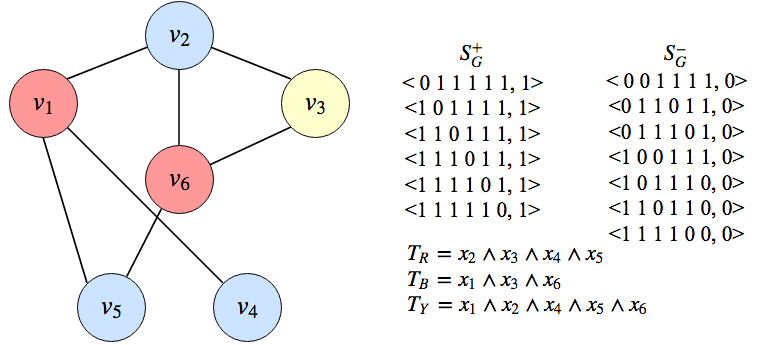
\includegraphics[width=\textwidth*7/8]{threecoloring.png}

\emph{A graph $G$ with a legal 3-coloring, the associated sample, and the terms defined by the coloring.}
\end{center}
\end{figure}
We now show that $G$ is 3-colorable iff $S_G$ is consistent with some $3$-term
DNF formula. Let us first consider the necessary condition. Suppose $G$ is
$3$-colorable and fix a $3$-coloring of $G$. Let $R$ be the set of all red
vertices, and let $T_R$ be the conjunction of all variables in $x_1, \dots, x_n$
whose index does \emph{not} appear in $R$. Therefore, for each $i \in R$, $v(i)$
must satisfy $T_R$. Additionally, no such $e(i,j) \in S_G^{-}$ can satisfy $T_R$.
Since $i$ and
$j$ can't both be colored red, at least $x_i$ or $x_j$ must be in $T_R$. We can
define terms for $T_B$ and $T_Y$ (blue, yellow) conjunctions in a similar fashion,
with no negative examples being accepted by any term.

We now show the other direction. Assume that the formula $T_R \vee T_B \vee T_Y$
is consistent with $S_G$. We define a 3-coloring of $G$: the color of the vertex
$i$ is red if $v(i)$ satisfies $T_R$, blue if $v(i)$ satisfies $T_B$, and yellow
if $v(i)$ satisfies $T_Y$. Break ties arbitrarily if $v(i)$ satisfies more than
one term. Since the formula is consistent with $S_G$, then every $v(i)$ must
satisfy some term and every vertex must be assigned a color.

We now prove that
this is a valid legal 3-coloring. Assume WLOG that two vertices $i$ and $j$ with
$(i \neq j)$ are given the same color, red. Then, both $v(i)$ and $v(j)$ satisfy
$T_R$. By the definition of $v(\cdot)$, the $i$th bit of $v(i)$ is 0 and the
$i$th bit of $v(j)$ is 1. Hence, neither $x_i$ nor $\neg x_i$ can appear in
$T_R$ - and the $i$th assignment does not affect the result of $T_R$. Since
$v(j)$ and $e(i,j)$ differ only in the $i$th bits, if $v(j)$ satisfies $T_R$,
then so does $e(i,j)$. This implies that $e(i,j) \not\in S_G^{-}$ and hence
$(i,j) \not\in E$.

We therefore observe that 3-term DNF formulae are not efficiently PAC learnable
under the following assumptions:
\begin{itemize}
    \item $NP$-complete problems cannot be solved with high probability by a
    probabilistic polynomial time algorithm
    \item the PAC learning algorithm is restricted to outputting a hypothesis
    from the same representation class as the target concept.
\end{itemize}

\end{proof}

\section{Using 3-CNF to Avoid Intractability}

If we relax the constraint on learning 3-term DNF formulae by expanding the
output hypothesis concept class to one that is more expressive, then the class
of 3-term DNF formula \emph{is} in fact efficiently PAC-learnable.

We first observe that any 3-term DNF formula over the variables
$x_1, \dots, x_n$ may be expanded to an equivalent 3-term CNF formula via
distributivity of $\vee$ over $\wedge$.

$$T_1 \vee T_2 \vee T_3 \equiv \bigwedge_{u \in T_1, v \in T_2, w \in T_3} (u \vee v \vee w)$$

We can reduce the problem of PAC learning 3-CNF formulae to the problem of PAC
learning conjunctions, which we saw in section $3$. Given an oracle for random
examples for some unknown target $3$-CNF formula, we can apply a transformation
to render each positive/negative example into a corresponding positive/negative
example over a larger set of variables. This transformation will render the
$3$-CNF formula as a simple boolean conjunction which we may efficiently
learn.

The transformation is as follows: for every triple of literals $u, v, w$ over
the original variable set $x_1, \dots, x_n$, the new variable set contains a
variable $y_{u,v,w} = u \vee v \vee w$. When $u = v = w$, $y_{u,v,w} = u$.
Hence, this expanded variable set fully contains all of the original variables.
The total number of new variables is thus $(2n)^3 = O(n^3)$.

Thus, for any assignment $a \in \{0, 1\}^n$ to the original variables
$x_1, \dots, x_n$, we can compute the corresponding assignment $a'$ to the new
variables $\big\{y_{u,v,w} | u, v, w \in \{x_1, \dots, x_n\}\big\}$ in $O(n^3)$
time. It is obvious that any 3-CNF formula over $x_1, \dots x_n$ is a simple
boolean conjunction over $y_{u, v, w}$. We can run the algorithm for learning
boolean conjunctions by expanding each assignment to $x_1, \dots, x_n$ that is a
positive example for the target formula to an assignment for the corresponding
$y_{u,v,w}$ and giving this expanded assignment to the algorithm as a positive
example for the unknown conjunction over $y_{u, v, w}$. When finished, we can
convert the hypothesis conjunction $h'$ back to a 3-CNF $h$ by expanding every
variable to its corresponding 3-term conjunction.

To conclude, we must argue that if $c$ and $\mathcal{D}$ are the target 3-CNF
formula and distribution over $\{0, 1\}^n$, and $c'$ and $\mathcal{D}'$ are the
corresponding conjunction over the $y_{u,v,w}$ and induced distribution over
assignments $a'$ to the $y_{u,v,w}$, then if $h'$ has error less than $\epsilon$
with respect to $c'$ and $\mathcal{D}'$, $h$ has error less than $\epsilon$ with
respect to $c$ and $\mathcal{D}$ as well. This is simple to see when noting that
the
applied transformation is injective. If $a_1$ is mapped to $a_1'$ and $a_2$ is
mapped to $a_2'$, then $a_1 \neq a_2$ implies $a_1' \neq a_2'$. Thus, each
assignment $a'$ on which $h'$ differs from $c'$ has a unique pre-image $a$ on
which $h$ differs from $c$, and the weight of $a$ under $\mathcal{D}$ is exactly
that of $a'$ under $\mathcal{D}'$. (Do note that the reduction exploits the
notion that the conjunctions learning algorithm works for any distribution
$\mathcal{D}$, as the transformation alters the original distribution).

Therefore, we have proven:\\

\begin{framed}
\begin{thm}
    The representation class of $3$-CNF formulae is efficiently PAC learnable.
\end{thm}
\end{framed}

Therefore, we can efficiently PAC-learn 3-term DNF formulae by rendering them as
3-CNF and allowing the hypothesis to be a 3-CNF formula. This does not hold if
we restrict the hypothesis class to 3-term DNF! As it turns out, this statement
holds for any constant $k \geq 2$ for $k$-term DNF formulae and $k$-CNF formulae.

It is critical to recognize that even with a fixed concept class from which
targets are chosen, the choice of \emph{hypothesis representation} can have a
huge impact on efficiency and tractability.

\section{Boosting}
In the problem of PAC-learnability, we were trying to find learning algorithms
that learned the problem really well - to within some $\epsilon$ error rate.
This is a pretty strong guarantee, so what if we have a problem where we can
only find an algorithm that does slightly better than random guessing? To
formalize this a little bit, let us define \emph{weak PAC-learning}.
Weak PAC-learning is largely the same as PAC-learning, except we alter the
learning condition to be (for a binary classification problem)
\begin{equation*}
    err_D(h) \leq \frac{1}{2} - \alpha.
\end{equation*}
for some $0 < \alpha < \frac{1}{2}$. Clearly, this is a much weaker guarantee than
the standard PAC-learning model, so we can call learning algorithms that are
successful under this model \emph{weak learners} and learning algorithms
successful under standard PAC-learning \emph{strong learners}. It is also easy
to see that a strong learner is also a weak learner. However, a somewhat
counterintuitive claim is that all weak learners are capable of strong learning.
How?

In knowledge-based game shows, a common ``lifeline'' to help out a contestant
is to let them ask the audience what they think the answer is and then that
contestant can use the most popular answer from the crowd as their answer. This
crowdsourcing idea can be quite powerful and we can do something similar with
weak learners. If you had a weak learner $\LL$, we could keep an
\emph{ensemble} of separate instances of $\LL$ and take the majority opinion
to be your classification. This would almost surely be better than a single weak
learner, but considering each ensemble member is still only a weak learner,
there is still a significant chance the
majority could be wrong. A natural improvement on this algorithm would be to
take a weighted majority by weighting the opinion of each member of the ensemble
based on its error rate, so that ``better'' members are weighted more highly.

We can do even better than this though. Using a technique called \emph{adaptive
boosting}, or AdaBoost for short, we have a guaranteed method of turning a weak
learner into a strong learner. You can read more about the AdaBoost algorithm
in Appendix E.

\appendix
\section{Appendix A: Agnostic Learning}
\textbf{Unrealizable case.} In the sample-bound analysis presented
earlier, we consider the case
where the target concept $c(x)$ always exists and $c \in \mathcal{C}$.
We call this the realizable case. In the \emph{unrealizable} situation,
such a $c$ may not exist. Hence, we may not be able to produce a
hypothesis that is perfectly consistent with a training set.

\emph{Agnostic learnability.} A concept class $\mathcal{C}$ is
agnostically learnable if $\exists$ a learning algorithm $\mathcal{L}$
such that $\forall c_t \in \mathcal{C}$, $\forall$ distributions
$\mathcal{D}$ over $\mathcal{X}$, and $\forall \epsilon, \delta > 0$,
and given some $\epsilon, \delta,$ and an oracle $EX(c_t, \mathcal{D})$,
$\mathcal{L}$ outputs an $h \in \mathcal{H}$ such that with probability
at least $1 - \delta$ it satisfies along with the efficiency conditions
for PAC-learning:

$$err_D(h) \leq \min_{h'\in \mathcal{C}} \hat{err_D}(h') + \epsilon$$

As a note, in various contexts you may see $min_{h' \in \mathcal{C}}
\hat{err}_D(h')$ written as $Opt(\mathcal{C})$ - the minimal empirical
error over all the possible hypotheses in $\mathcal{C}$.

The idea is that we want an algorithm that minimizes true error despite
that the true errors of the functions in $C$ are unknown.

As before, we want to identify a sufficient sample size $m$ that will
let a learning algorithm produce a minimal error hypothesis. First,
we'll show that for any particular $h$, the empirical and true errors
converge. Then, we'll show that the errors converge for all $h \in
\mathcal{C}$ - thus, minimizing $\hat{err}_D(h)$ over all $h \in
\mathcal{C}$ will approximately minimize $err_D(h)$.

\emph{Claim.} Let $h$ be a function $h\;:\;\mathcal{X}\rightarrow
\mathcal{Y} = \{0,1\}$. Then, $$P(|\hat{err_D}(h) - err_D(h)| \geq
\epsilon) \leq 2e^{-2\epsilon^2 m}$$ for any probability distribution
$\mathcal{D}$, any $\epsilon >0$, and any positive integer $m$.

\begin{proof}
    Consider the indicator function $f_i(x_i)$,
    $$f_i(x_i) = \begin{cases}
        1&\text{ if $h(x_i) \neq y_i$}\\
        0&\text{ otherwise}
    \end{cases}$$

    Then, we can define the empirical error - the probabiliy that $h$
    misclassifies a point over the examples.

    $$\hat{err}_D(h) = \frac{1}{m}\sum_{i=1}^m f_i(x_i)$$

    Finally, we define true error as: $$err_D(h) = E_{X\sim D}[f_i(x)]$$

    Using the Hoeffding inequality (see Appendix A), we can then write:

    $$P(|\hat{err_D}(h) - err_D(h)| \geq \epsilon) \leq 2 e^{-2\epsilon^2 m}$$

    This concentration inequality tells us that with larger sample size
    $m$, the empirical error exponentially rapidly approaches the true
    error.

\end{proof}

The above claim gives a bound on the difference between empirical and
true error for a particular hypothesis $h$. We now bound the difference
between the errors for all $h \in \mathcal{C}$.

\emph{Claim.} $P(\exists h \in \mathcal{C}\;:\; |err_D(h) - \hat{err}_D(h)| \geq \epsilon) \leq 2 |\mathcal{C}|e^{-2\epsilon^2 m}$

\begin{proof}
    The claim immediately follows from the union bound:
    \begin{align*}
        P(\exists h \in \mathcal{C}\;:\; |err_D(h) - \hat{err}_D(h)|
        \geq \epsilon) &= P(\bigcup_{h\in\mathcal{C}} \bigg\{ |err_D(h)
        - \hat{err}_D(h)| \geq \epsilon \bigg\})\\
        &\leq \sum_{h\in \mathcal{C}} P(|err_D(h) - \hat{err}_D(h)| \geq \epsilon)\\
        &\leq 2|\mathcal{C}|e^{-2\epsilon^2 m}
    \end{align*}
\end{proof}

We set $\delta \geq 2|\mathcal{C}|e^{-2\epsilon^2 m}$. This way, we
upper bound the probability of any $h$'s true and empirical errors not
converging. Solving for $m$,

\begin{align*}
    \delta &\geq 2|\mathcal{C}|e^{-2\epsilon^2 m}\\
    \ln \delta &\geq \ln 2|\mathcal{C}| - 2\epsilon^2 m\\
    2\epsilon^2 m &\geq \ln 2 |\mathcal{C}| - \ln \delta\\
    m &\geq \frac{\ln 2 |\mathcal{C}| + \ln \frac{1}{\delta}}{2\epsilon^2}
\end{align*}

Looking at the equation obtained for finding an appropriate $m$, we
observe that the sample size depends on $\epsilon^2$ as opposed to
$\epsilon$ in the PAC-learning case. Thus, in practice when we cannot
find a consistent hypothesis, we need more data to obtain a hypothesis
with less true error.

Equivalently, given some number $m$ of examples, the error we expect is,
with probability at least $1 - \delta$,
$$err_D(h) \leq \hat{err}_D(h) + O\bigg(\sqrt{\frac{\ln(2|\mathcal{C}|)
+ \ln(\frac{1}{\delta})}{m}}\bigg)$$

From this, we can derive three core conditions for learning:

\begin{itemize}
    \item \emph{large amount of training data} - by increasing $m$, the
    second term becomes smaller, decreasing the total error
    \item \emph{low training error} - the first term in the summation -
    decreasing training error consequently decreases the true error
    \item \emph{simple hypothesis space} - the measure for simplicity
    here is the size of the hypothesis class. The smaller the hypothesis,
    the lower the true error
\end{itemize}

Additionally, there is a trade-off between decreasing training error and
maintaining a simple hypothesis. As the complexity of the hypotheses
increases, the probability of finding a consistent hypothesis increases
and the training error tends to zero. However, the big-Oh term will
eventually begin to dominate, and after $err_D(h)$ reaches a minimum, it
will begin to rise again. At this point, we have \emph{overfitting}, and
while the hypothesis chosen is consistent on the
training data, the variance introduced is too high! Complex hypotheses
assume more about the data ``from thin air'' without actual training data
to support the complexity.

\begin{center}
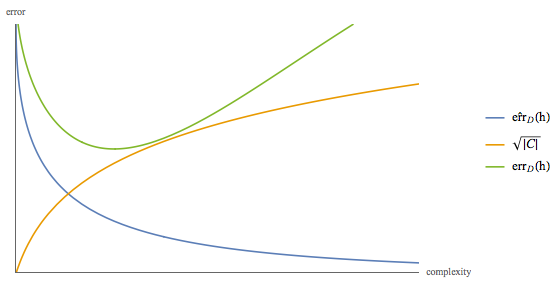
\includegraphics[width=\textwidth*6/8]{overfitting.png}

\emph{empirical error vs. true error}
\end{center}

Overfitting is one of the most difficult and most important issues to
deal with in practical machine learning. Often times, only the training
error $\hat{err_D}(h)$ can be observed directly, making it difficult to
minimize the other term. Here are a couple of main approaches towards
solving the overfitting problem:

\begin{itemize}
    \item \emph{Structural Risk Minimization (SRM)}: an inductive
    principle for model selection. Select from a set of models in order
    of increasing complexity - pick one for which the sum of empirical
    risk and complexity (VC-dimension) is minimal. The goal is to find
    the exact value of the theoretical bounds to minimize the bound
    directly.
    \item \emph{Cross-Validation}: Separate training data into two
    parts: a training and a testing set. This lets us estimate the true
    error and identify the stopping point for the algorithm (i.e. when
    the true error reaches a minimal point). Variations on this include
    splitting the data into $k$ parts ($k$-fold CV), or trying the
    algorithm on all data points except one and repeating (LOOCV).
\end{itemize}

As a side note (this is outside the scope of this lecture),
this theorem can actually be generalized to
infinite classes. But then wouldn't the number of samples
needed just be infinity, you ask? Actually, no! We can use
something called the Vapnik-Chervonenkis dimension, which
is the largest dimension in which all labels of points can
be induced by functions in $\mathcal{C}$. Appendix B further explores
the notion of VC dimension. Using this concept gives
us the following theorem:\\

\begin{framed}
\begin{thm}
    If you find an algorithm that is consistent given
    $m \geq \frac{VCD(\mathcal{C})}{\epsilon}\ln(\frac{1}{\delta})$ samples,
    then with probability $1-\delta$ it satisfies the
    learning condition.
\end{thm}
\end{framed}

\section{Appendix B: Jensen's and Hoeffding's Inequalities}

\textbf{Jensen's Inequality.} Jensen's inequality is arguably one of the most
significant inequalities in all of statistics, and we will in fact use it later
to prove Hoeffding's lemma. The inequality relates the convex function of an
expectation to the expectation of the convex function. We first briefly review
important properties of convex functions.

\emph{Convex function.} Let $I$ be an open subset of $\mathbb{R}$.
Let $f\;:\;I\rightarrow \mathbb{R}$. We say that $g$ is \textbf{convex} if
$\forall x_1, x_2 \in I$ and $\forall t \in [0, 1]$ we have
$$f(t x_1 + (1-t) x_2) \leq t f(x_1) + (1-t)f(x_2)$$

In layman's terms, this means that the value of a convex function evaluated at a
value in the range $[x_1, x_2]$ is always bounded above by a point through the
secant line through $f(x_1)$ and $f(x_2)$.

\begin{center}
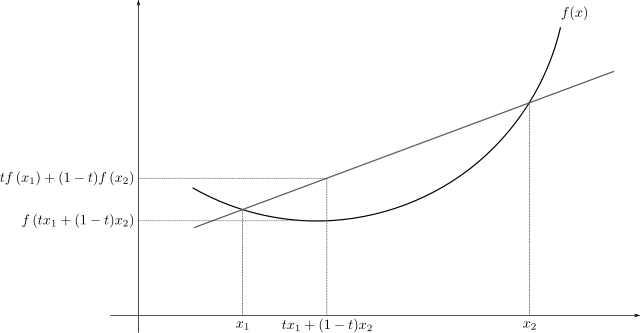
\includegraphics[width=\textwidth*6/8]{convexfunction.png}
\end{center}

We can also define convex functions in more familiar terms:

\begin{lemma} (Sufficient conditions for convexity)

Let $I$ be an open subset of $\mathbb{R}$. Let $f\;:\;I\rightarrow \mathbb{R}$.
If either
\begin{enumerate}
    \item $f'$ is nondecreasing and continuous on $I$, or
    \item $f'' \geq 0$ on $I$
\end{enumerate}
then $f$ is convex.
\end{lemma}

Before we prove Jensen's inequality, we will prove the following useful property
of convex functions.

\begin{lemma}
    If $\psi$ is a convex function on the open subset $I \subset \mathbb{R}$,
    then for any $x_0 \in I$ there exists a support line $l_0$ such that
    $$l_0(x) \leq \psi(x)\;\forall x \in I\text{ and } l_0 (x_0) = \psi(x_0)$$
\end{lemma}

This means that for any function that is convex on a given interval, the
function lies above its tangent lines at any point in the interval.

\begin{proof}
We first observe two facts:
\begin{enumerate}
    \item For any $h > 0$, we have $$\frac{\psi(x)-\psi(x-h)}{h} \leq \frac{\psi(x+h)-\psi(x)}{h}$$
    We can obtain this result from the definition of convexity:
    \begin{align*}
        \psi(t(x-h) + (1-t)(x+h)) &\leq t\psi(x-h) + (1-t)\psi(x+h)\\
        \psi(x) &\leq \frac{1}{2}\psi(x-h)+\frac{1}{2}\psi(x+h)&&\text{letting $t = \frac{1}{2}$}\\
        \psi(x)-\psi(x-h) &\leq \psi(x+h)-\psi(x)\\
    \end{align*}
    Dividing both sides by the constant $h$ gives us the desired result. $(1)$
    effectively states that a right derivative will always be larger than a left
    derivative for a convex function.

    \item For any $h_1 > h_2$,
        $$\frac{\psi(x)-\psi(x-h_1)}{h_1} \leq \frac{\psi(x)-\psi(x-h_2)}{h_2}$$
        $$\frac{\psi(x+h_1) - \psi(x)}{h_1} \geq \frac{\psi(x+h_2)-\psi(x)}{h_2}$$
    We obtain the first inequality from the definition of convexity where $t = \frac{h2}{h1}$, and the points are $x-h_1$ and $x$.
    \begin{align*}
        \psi(\frac{h_2}{h_1}(x-h_1)+(1-\frac{h_2}{h_1})x) &\leq \frac{h_2}{h_1}\psi(x-h_1) + (1-\frac{h_2}{h_1})\psi(x)\\
        \psi(x-h_2) &\leq \frac{h_2}{h_1}\psi(x-h_1) + \psi(x) -\frac{h_2}{h_1}\psi(x)\\
        \frac{h_2}{h_1}\psi(x) - \frac{h_2}{h_1}\psi(x-h_1) &\leq \psi(x) - \psi(x-h_2)\\
        \frac{\psi(x)-\psi(x-h_1)}{h_1} &\leq \frac{\psi(x)-\psi(x-h_2)}{h_2}
    \end{align*}

    The second inequality may be found in a similar fashion, except using the
    points $x+h_1$ and $x$.
\end{enumerate}

By $(2)$, we observe that the sequences are monotone. This directly leads from
the fact that for a convex function, the derivative is always increasing. Thus,
their limits as $h \rightarrow 0^{+}$ exist by the Monotone Convergence Theorem.
We then define:
$$\psi'_{-}(x) = \lim_{h\rightarrow 0^{+}} \frac{\psi(x)-\psi(x-h)}{h} \text{ and } \psi'_{+}(x) = \lim_{h\rightarrow 0^{+}} \frac{\psi(x+h)-\psi(x)}{h}$$

By $(1)$, we have that $\psi'_{-}(x) \leq \psi'_{+}(x)$ for any $x$. Then, for
fixed $z$, we can choose some $m \in [\psi'_{-}(z), \psi'_{+}(z)]$ and define
the line $\ell$,
$$\ell_z(x) = \psi(z)+m(x-z)$$

We thus have $\ell_z(z) = \psi(z)$. If we consider any $x = z + h$ for some $h$,
it is easy to see that the inequality
$\ell_z(z+h) = \psi(z) + m h \leq \psi(z + h)$ holds.
(Hint: observe the notion that $\psi'(x)$ monotonically increases).
\end{proof}

We now state Jensen's inequality.

\begin{framed}
\begin{thm} (Jensen's Inequality)
Let $f$ be a convex function on $I$, an open subset of $\mathbb{R}$.
Let $x \in I$ with probability $1$ and assume $X, f(X)$ have finite expectation.
Then $$f(EX) \leq E[f(X)]$$
\end{thm}
\end{framed}

\begin{proof}
First, we observe that $EX \in I$. Let $\ell(x) = ax + b$ be the support line
for $f(\cdot)$ at the point $EX$. Then, by the definition of the support line we
have
\begin{enumerate}
    \item $\ell(EX) = f(EX)$
    \item $\ell(x) \leq f(x)\;\forall x \in I$
\end{enumerate}

Taking expectations in $(2)$, we have:
$$E[f(x)] \geq E[\ell(x)] = E[ax + b] = a E[x] + b = \ell(EX)$$

Then invoking $(1)$, we have $E[f(x)] \geq f(EX)$ and are done.
\end{proof}

\textbf{Hoeffding's Inequality.} Hoeffding's inequality is one of the most
important inequalities in machine learning literature. It gives an
\textbf{exponential} bound for sums of random variables whose intervals are
bounded. Before introducing and proving Hoeffding's inequality, we first
introduce the following lemma.

\begin{lemma}
    Let $a, b$ be constants such that $a \leq 0, 0 \leq b, a \neq b$. Let $X$
    be any real valued random variable such that $EX = 0$ and $a \leq X \leq b$.
    For all $\lambda \in \mathbb{R}$,
    $$E[e^{\lambda X}] \leq \exp(\frac{\lambda^2(b-a)^2}{8})$$
\end{lemma}

\begin{proof}

We first consider the moment generating function $e^{\lambda X}$. Since this is
a convex function, we may use the fact that $a \leq X \leq b$ to invoke Jensen's
inequality for two points (which is just the definition of a convex function):
$$f(t a + (1-t)b) \leq t f(a) + (1-t)f(b)$$

Parameterizing $x$ with respect to $t \in [0, 1]$, we set $x = ta + (1-t)b$ and
have $ t = \frac{b-x}{b-a}$. Then,
$$e^{\lambda x} \leq \frac{b-x}{b-a} e^{\lambda a} + \frac{x-a}{b-a}e^{\lambda b}.$$

Taking expectation with respect to $x$, we have:

\begin{align*}
    E[e^{\lambda x}] &\leq \frac{b - EX}{b-a}e^{\lambda a} + \frac{EX - a}{b-a}e^{\lambda b}\\
        &= \frac{b}{b-a} e^{\lambda a} - \frac{a}{b-a} e^{\lambda b}
\end{align*}

Let $h = \lambda(b-a), p = \frac{-a}{b-a}, L(h) = -hp + \ln(1-p+pe^h)$.

We then substitute our values,
\begin{align*}
    E[e^{\lambda x}] &\leq (1-p)e^{\lambda a} + pe^{\lambda b}\\
        &\leq (1-p)e^{-hp} + pe^{h(1-p)}\\
        &\leq (1-p+pe^h)e^{-hp}\\
        &= e^{L(h)}
\end{align*}

To complete the proof, we will show $L(h) \leq \frac{1}{8}\lambda^2(b-a)^2$.

We first compute $L'(h)$ and $L''(h)$. With simple calculus,
$$L'(h) = -p + \frac{1}{1-p+pe^h} pe^h$$
$$L''(h) = \frac{1}{1-p+pe^h}pe^h - (pe^h)^2(\frac{1}{1-p+pe^h})^2$$

Showing the first few terms of the Taylor expansion of $e^{L(h)}$,
\begin{align*}
    L(h) \approx L(0) + L'(0) h + \frac{L''(0)}{2!} h^2 + \dots
\end{align*}

We note that $L(0) = L'(0) = 0$. We note that since the dominant term in $L(h)$
is of the form $\ln(1-u)$, a finite Taylor expansion for $L$ will always be an
overestimate. Thus, $L(h) \leq \frac{L''(0)}{2} h^2$. We then show that $L''(0)
\leq \frac{1}{4}$.

Simplifying and evaluating $L''(0)$ is a bit messy.

We first simplify $1 - p + pe^h = 1 + \frac{a}{b-a} - \frac{a}{b-a}e^h = \frac{b-ae^h}{b-a}$.
\begin{align*}
    L''(h) &= (\frac{1}{1-p+pe^h})p e^h - (\frac{1}{1-p+pe^h})^2 (pe^h)^2\\
            &= \frac{pe^h(1-p+pe^h)-(pe^h)^2}{(1-p+pe^h)^2}\\
            &= \frac{(b-a)^2 [\frac{-a}{b-a}e^h(\frac{b-ae^h}{b-a})-e^{2h}\frac{a^2}{(b-a)^2}]}{(b-ae^h)^2}\\
            &= \frac{-a e^h (b-ae^h) - e^{2h} a^2}{(b-ae^h)^2}\\
            &= \frac{-bae^h + e^{2h}a^2 - e^{2h}a^2}{(b-ae^h)^2}\\
            &= \frac{-bae^h}{(b-ae^h)^2}
\end{align*}

Evaluating at $h = 0$, we have
\begin{align*}
    L''(0) = \frac{-ba}{(b-a)^2} &\leq \frac{1}{4}\\
            -4ba &\leq b^2 -2ab + a^2\\
            0 &\leq b^2 + 2ab + a^2 = (b+a)^2
\end{align*}

This is clearly always true, and we therefore have
$$E[e^{\lambda x}] \leq e^{L(h)} = e^{\frac{1}{8} h^2} = e^{\frac{1}{8} \lambda^2 (b-a)^2}$$
\end{proof}

\begin{framed}
\begin{thm} (Hoeffding's Inequality.) Let $X_1, \dots, X_n$ be independent
random variables bounded such that $X_i \in [a_i, b_i]$.
$$P(\bar{X} - E\bar{X} \geq t) \leq \exp\bigg(-\frac{2n^2t^2}{\sum_{i=1}^n (b_i-a_i)^2}\bigg)$$
\end{thm}
\end{framed}

\begin{proof}
Suppose that $X_1, \dots, X_n$ are $n$ independent random variables such that
$$P(X_i \in [a_i, b_i]) = 1$$ for $1 \leq i \leq n$. Let $S_n = X_1 + \cdots + X_n$.
Then for $s, t \geq 0$, we can invoke Markov's inequality:

\begin{align*}
    P(S_n - E[S_n] \geq t) &= P(e^{s(S_n-E[S_n])} \geq e^{st})\\
        &\leq e^{-st} E[e^{s(S_n - E[S_n])}]&&\text{ Markov's inequality}\\
        &= e^{-st} \prod_{i=1}^n E[e^{s(X_i-E[X_i])}]&&\text{ Expectation of product of indep. R.V.s}\\
        &\leq e^{-st} \prod_{i=1}^n \exp(\frac{1}{8} s^2(b_i - a_i)^2)&&\text{ Hoeffding's Lemma}\\
        &= \exp(-st + \frac{1}{8} s^2 \sum_{i=1}^n (b_i - a_i)^2)
\end{align*}

To find the tightest upper bound, we want to minimize the right hand side of the
last inequality as a function of $s$. We define $g(s) = -st + \frac{s^2}{8}\sum_{i=1}^n(b_i - a_i)^2$.

Since $g$ is a quadratic function of $s$, we can solve $g'(s) = 0$ to find the minimum:
$$s = \frac{4t}{\sum_{i=1}^n (b_i-a_i)^2}$$

Plugging back in to $g(s)$, we get the tight bound:
$$P(S_n - E[S_n] \geq t) \leq \exp\bigg(-\frac{2t^2}{\sum_{i=1}^n(b_i-a_i)^2}\bigg)$$

If we define some $\bar{X} = \frac{S_n}{n}$, we can rewrite the above to get the
form shown in the theorem.

\end{proof}

In the special case where $a_i = 0$ and $b_i = 1$, we have:
$$P(\bar{X} - E[\bar{X}] \geq t) \leq e^{-nt^2}$$

This form is particularly important, as it is applied to the case of i.i.d.
Bernoulli random variables often in computer science.

\section{Appendix C: VC-Dimension}

In our foray into learning algorithms, we only considered cases where the
hypothesis classes chosen were of finite size. However, this is a significant
limitation - and often times we will want to consider hypothesis classes of
infinite cardinality.

In the inequalities for $err_D(h)$ obtained in both the PAC-learning and
agnostic learning cases, we have terms containing $\ln(|\mathcal{C}|)$. If
$\mathcal{C}$ is of infinite cardinality, we effectively have an infinite upper
bound on the true error, which is useless! We instead introduce the notion of
the Vapnik-Chervonenkis dimension measure - even though $\mathcal{C}$ may have
infinite cardinality, the restriction of the application of concepts in
$\mathcal{C}$ to a finite sample $S$ has a finite outcome.

As before, we assume that $\mathcal{C}$ is a concept class over the instance
space $\mathcal{X}$, both of which may be infinite. We define each
$c \in \mathcal{C}$ such that $c\;:\;\mathcal{X} \rightarrow \{0,1\}$
(i.e. positive or negative labels). A training sample $S$ of $m$ samples $x_1,
\dots, x_m$ is drawn i.i.d. according to some fixed but unknown distribution $D$.
We further reserve $c \in \mathcal{C}$ to denote the target concept and
$h \in \mathcal{C}$ to denote an arbitrary concept.

\textbf{Dichotomies on $S$.}
$$\Pi_\mathcal{C}(S) = \{(h(x_1),\dots,h(x_m)\;:\;h\in \mathcal{C}\},$$
    where $\Pi_\mathcal{C} \in \{0,1\}^m$.

$\Pi_\mathcal{C}(S)$ is a set whose members are $m$-dimensional boolean vectors
\emph{induced} by concepts in $\mathcal{C}$. We refer to these members as
\emph{dichotomies} or \emph{behaviors} on $S$ induced or realized by
$\mathcal{C}$. We say that $\mathcal{C}$ fully realizes $S$ if
$|\Pi_\mathcal{C}(S)| = 2^m$ - that is, every possible $m$-dimensional boolean
vector can be obtained by passing $S$ through all concepts $h \in \mathcal{C}$.

Equivalently, $\Pi_\mathcal{C}(S)$ can be represented as a collection of subsets
of $S$: $$\Pi_\mathcal{C}(S) = \{h \cap S\;:\;h\in \mathcal{C}\},$$ where each
$h\in\mathcal{C}$ makes a partition of $S$ into two sets, the positive and
negative points. We say that $h \cap S$ yields a subset of $S$ containing the
positive points of $S$ under $h$. Under this representation, $\mathcal{C}$ fully
realizes $S$ when the total number of $h \cap S$ = $2^m$ for all
$h \in \mathcal{C}$. We can view this as taking the sum
$\sum_{i=0}^m \binom{m}{i}$, the total number of ways of picking any number
$0 \leq i \leq m$ of the points to be labeled positive.

\textbf{Shattering.} If $|\Pi_\mathcal{C}(S)| = 2^m$, then $S$ is considered
\textbf{shattered} by $\mathcal{C}$. In other words, $S$ is shattered by
$\mathcal{C}$ if $\mathcal{C}$ fully realizes $S$.

\emph{Example.} Consider the finite concept class
$\mathcal{C} = \{c_1, \dots, c_4\}$ applied to three instance vectors
$\mathbf{x_1, x_2, x_3}$ with the results:

\begin{center}
\begin{tabular}{c|c c c}
    &$\mathbf{x_1}$&$\mathbf{x_2}$&$\mathbf{x_3}$\\\hline
    $c_1$&$1$&$1$&$1$\\
    $c_2$&$0$&$1$&$1$\\
    $c_3$&$1$&$0$&$0$\\
    $c_4$&$0$&$0$&$0$
\end{tabular}
\end{center}

\begin{align*}
    \Pi_\mathcal{C}(\{\mathbf{x_1}\}) &= \{(0),(1)\}&&\text{shattered}\\
    \Pi_\mathcal{C}(\{\mathbf{x_1, x_3}\}) &= \{(1,1), (0, 1), (1, 0), (0, 0)\}&&\text{shattered}\\
    \Pi_\mathcal{C}(\{\mathbf{x_2, x_3}\}) &= \{(1,1), (0,0)\}&&\text{not shattered}
\end{align*}

In the final case, choosing $S = \{\mathbf{x_2, x_3}\}$ only yields $2$ of the
$4$ possible dichotomies of $S$. We now finally define VC dimension.\\

\begin{framed}
\textbf{Vapnik-Chervonenkis Dimension}. The VC dimension of the concept class
$\mathcal{C}$, denoted as $VCdim(\mathcal{C})$, is the cardinality of the
largest set $S$ shattered by $\mathcal{C}$. If all sets $S$ that are arbitrarily
large can be shattered by $\mathcal{C}$, then $VCdim(\mathcal{C}) = \infty$.
\end{framed}

We observe that the VC dimension of a concept class is a
\emph{combinatorial measure of its complexity.} We can interpret the VC
dimension as the point $d$ at which all samples $S$ with complexity $|S| > d$
can no longer be shattered by $\mathcal{C}$. In other words, for all
$h \in \mathcal{C}$, it is not possible to obtain all possible results
(dichotomies)! Intuitively, this marks the VC dimension as a good metric for
complexity, as it tells us at which point a concept class
exhausts its capacity to fully realize all results for the input.

As an important note, it is crucial to realize that if the VC dimension is at
least $d$, then this means that there \emph{exists} some sample $|S| = d$ that
is shattered by $\mathcal{C}$. This does not imply that all samples of size $d$
are shattered by $\mathcal{C}$. Conversely, to show that the VC dimension is at
most $d$, one must show that no sample of size $d+1$ can be shattered by
$\mathcal{C}$.

We now look at an example concept-class and its VC dimension.

\textbf{Intervals on the Reals.} The concept class $\mathcal{C}$ is governed by
two parameters $\alpha_1, \alpha_2$ in the closed interval $[0, 1]$. A concept
from the class will label an input instance $0 < x < 1$ as positive if
$\alpha_1 \leq x \leq \alpha_2$ and negative otherwise. We show that the VC
dimension is at least $2$. Select any sample of $2$ points $x_1, x_2$ positioned
in the open interval $(0,1)$. It is clear that one can pick values of
$\alpha_1, \alpha_2$ to produce all
the possible four dichotomies $(+, +), (-, -), (+, -), (-, +)$. \\

\begin{center}
\emph{$(-, -)$ Case}

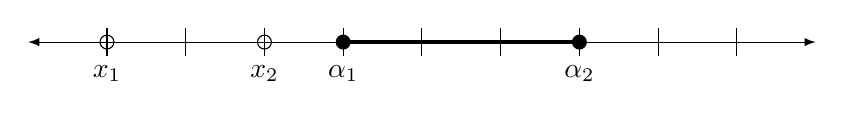
\begin{tikzpicture}[scale=10]
\draw[latex-latex] (0, 0) -- (1.0, 0);
\foreach \x in {0.1, 0.2,...,0.9}
    \draw[shift={(\x,0)}, color=black] (0pt, 0.5pt) -- (0pt, -0.5pt);
\draw[*-*] (0.392, 0) -- (0.708, 0);
\draw[very thick] (0.392, 0) -- (0.708, 0);
\draw[] (0.4, 0) circle(0.25pt) node[below=5pt] {$\alpha_1$};
\draw[] (0.7, 0) circle(0.25pt) node[below=5pt] {$\alpha_2$};
\draw[] (0.1, 0) circle(0.25pt) node[below=5pt] {$x_1$};
\draw[] (0.3, 0) circle(0.25pt) node[below=5pt] {$x_2$};
\end{tikzpicture}

\emph{$(-, +)$ Case}

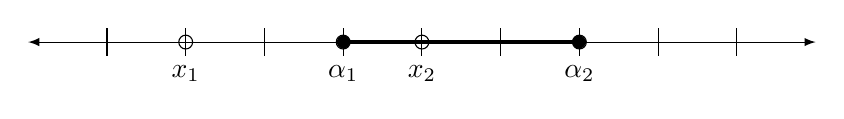
\begin{tikzpicture}[scale=10]
\draw[latex-latex] (0, 0) -- (1.0, 0);
\foreach \x in {0.1, 0.2,...,0.9}
    \draw[shift={(\x,0)}, color=black] (0pt, 0.5pt) -- (0pt, -0.5pt);
\draw[*-*] (0.392, 0) -- (0.708, 0);
\draw[very thick] (0.392, 0) -- (0.708, 0);
\draw[] (0.4, 0) circle(0.25pt) node[below=5pt] {$\alpha_1$};
\draw[] (0.7, 0) circle(0.25pt) node[below=5pt] {$\alpha_2$};
\draw[] (0.2, 0) circle(0.25pt) node[below=5pt] {$x_1$};
\draw[] (0.5, 0) circle(0.25pt) node[below=5pt] {$x_2$};
\end{tikzpicture}

\emph{$(+, -)$ Case}

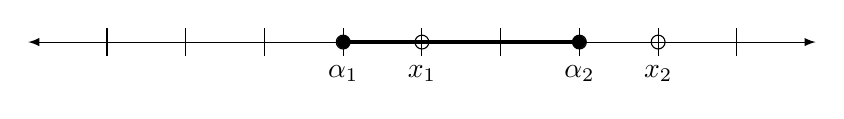
\begin{tikzpicture}[scale=10]
\draw[latex-latex] (0, 0) -- (1.0, 0);
\foreach \x in {0.1, 0.2,...,0.9}
    \draw[shift={(\x,0)}, color=black] (0pt, 0.5pt) -- (0pt, -0.5pt);
\draw[*-*] (0.392, 0) -- (0.708, 0);
\draw[very thick] (0.392, 0) -- (0.708, 0);
\draw[] (0.4, 0) circle(0.25pt) node[below=5pt] {$\alpha_1$};
\draw[] (0.7, 0) circle(0.25pt) node[below=5pt] {$\alpha_2$};
\draw[] (0.8, 0) circle(0.25pt) node[below=5pt] {$x_2$};
\draw[] (0.5, 0) circle(0.25pt) node[below=5pt] {$x_1$};
\end{tikzpicture}

\emph{$(+, +)$ Case}

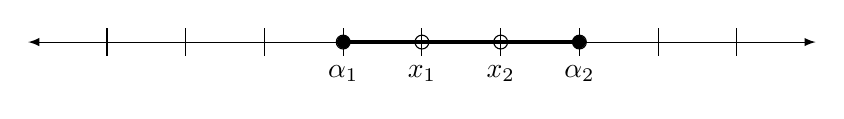
\begin{tikzpicture}[scale=10]
\draw[latex-latex] (0, 0) -- (1.0, 0);
\foreach \x in {0.1, 0.2,...,0.9}
    \draw[shift={(\x,0)}, color=black] (0pt, 0.5pt) -- (0pt, -0.5pt);
\draw[*-*] (0.392, 0) -- (0.708, 0);
\draw[very thick] (0.392, 0) -- (0.708, 0);
\draw[] (0.4, 0) circle(0.25pt) node[below=5pt] {$\alpha_1$};
\draw[] (0.7, 0) circle(0.25pt) node[below=5pt] {$\alpha_2$};
\draw[] (0.6, 0) circle(0.25pt) node[below=5pt] {$x_2$};
\draw[] (0.5, 0) circle(0.25pt) node[below=5pt] {$x_1$};
\end{tikzpicture}
\end{center}

To show that the VC dimension is at most $2$, it suffices to show that
\emph{any} sample $x_1, x_2, x_3$ on the line $(0, 1)$ cannot be shattered by
$\mathcal{C}$. We note that the dichotomy $(+, -, +)$ can never be realized by
any satisfying sample.\\

\begin{center}
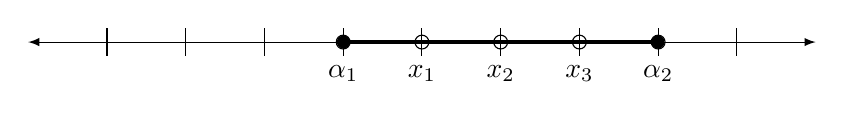
\begin{tikzpicture}[scale=10]
\draw[latex-latex] (0, 0) -- (1.0, 0);
\foreach \x in {0.1, 0.2,...,0.9}
    \draw[shift={(\x,0)}, color=black] (0pt, 0.5pt) -- (0pt, -0.5pt);
\draw[*-*] (0.392, 0) -- (0.808, 0);
\draw[very thick] (0.392, 0) -- (0.808, 0);
\draw[] (0.4, 0) circle(0.25pt) node[below=5pt] {$\alpha_1$};
\draw[] (0.8, 0) circle(0.25pt) node[below=5pt] {$\alpha_2$};
\draw[] (0.5, 0) circle(0.25pt) node[below=5pt] {$x_1$};
\draw[] (0.6, 0) circle(0.25pt) node[below=5pt] {$x_2$};
\draw[] (0.7, 0) circle(0.25pt) node[below=5pt] {$x_3$};
\end{tikzpicture}
\end{center}

We apply labels WLOG such that $x_1 < x_2 < x_3$. As shown above, if $x_1$ and
$x_3$ are both classified as $+$, i.e. both points are in the range
$[\alpha_1, \alpha_2]$, then $x_2$ must also be in the range and therefore
classified $+$. Therefore, it is not possible to obtain the dichotomy
$(+, -, +)$ from $\mathcal{C}$, and the VC dimension of $\mathcal{C}$ is $2$.

\section{Appendix D: Occam Learning}
% TODO

\section{Appendix E: AdaBoost}
Using a technique called \emph{adaptive boosting}, or AdaBoost for short, we
have a guaranteed method of turning a weak learner into a strong learner. We
can begin by calling our weak-learning algorithm $\LL$ to obtain a hypothesis
$h_1$. Now we can modify our original distribution $\mathcal{D}$ to create
$\mathcal{D}_2$, where we have reweighted the distribution to slightly favor
those samples that $h_1(x)$ classified incorrectly. We can do this again,
except use a $\mathcal{D}_3$ where those samples for which $h_1$ differs from
$h_2$ have higher weight. After repeating this for $T$ iterations, we have
produced $T$ hypotheses to use as our ensemble.

Why does this make sense? Well, if we reweight our distribution to favor samples
that our hypothesis was wrong on such that the hypothesis is no better than
random guessing and then rerun our learning algorithm, we know it has to perform
better than random guessing so our algorithm must learn some hypothesis that
performs better on the samples the first hypothesis erred on.

This means that we will have a set of hypotheses, each of which perform better
on different areas of the sample space. Thus we can output a final output that
weights each of these hypotheses:
\begin{equation*}
    H(x) = sign\left(\sum_{i = 1}^{T} \alpha_i h_i(x)\right).
\end{equation*}
The creation of the AdaBoost algorithm, below, specified exactly how to
calculate the weights $\alpha_i$ and generate the new distribution $D_{t+1}$.

\begin{figure}[H]
\begin{framed}
    \begin{algorithmic}
        \State $D_1 \leftarrow \frac{1}{n}$ for $i \leftarrow 1,\ldots, n$
        \For{$t \leftarrow 1,\ldots, n$}
            \State Produce hypothesis $h_t$ from distribution $D_t$
            \State Let $\epsilon_t = Pr_{i\sim D_t} [h_t(x_i) \neq y(x_i)]$
            \State Let $\alpha_t = \frac{1}{2}\ln\left(\frac{1 -
            \epsilon_t}{\epsilon_t}\right)$
            \For{$i \leftarrow 1,\ldots, n$}
            \State $D_{t+1}(i) = \frac{D_{t}(i)}{z}e^{-\alpha_t h_t(x_i)
            y(x_i)}$, where $z$ is a normalization
            \State constant to enforce $D$ to be a distribution.
            \EndFor
        \EndFor
        \State 
        \State Output $H(x) = sign\left(\sum_{i = 1}^{T} \alpha_i h_i(x)\right)$
    \end{algorithmic}
\end{framed}
\begin{center}
    \emph{The AdaBoost algorithm.}
\end{center}
\end{figure}

In this current form, however, it can be quite computationally inefficient to
perform this algorithm because of all the logarithms and exponentials. With
some mathematical manipulations, however, we can make this much more efficient.

We can begin by rewriting $\alpha_t$:
\begin{equation*}
    \alpha_t = \frac{1}{2}\ln\left(\frac{1 - \epsilon_t}{\epsilon_t}\right) = 
    \ln\left(\sqrt{\frac{1 - \epsilon_t}{\epsilon_t}}\right)
\end{equation*}
Next, we can plug the value of $\alpha_t$ into the equation for $D_{t+1}(i)$:

\begin{align*}
    D_{t+1}(i) &= \frac{D_{t}(i)}{z}e^{-\ln\left(\sqrt{\frac{1 -
    \epsilon_t}{\epsilon_t}}\right)h_t(x_i) y(x_i)} \\
    &= \frac{D_{t}(i)}{z} * \begin{dcases} 
        \sqrt{\frac{\epsilon_t}{1 - \epsilon_t}}, 
            & \text{if } h_t(x_i)y(x_i) = 1 \\ 
        \sqrt{\frac{1 - \epsilon_t}{\epsilon_t}},
            & \text{if } h_t(x_i)y(x_i) = -1
    \end{dcases}
\end{align*}
Note that $h_t(x_i)y(x_i) = 1$ iff the hypothesis $h_t$ is correct for sample
$x_i$ and $-1$ if it is incorrect.

We can now work on finding an expression for $z$. We know that it is the
normalizing constant, so therefore:
\begin{equation*}
    z = \sqrt{\frac{\epsilon_t}{1 - \epsilon_t}} \sum_{\{i | h_t(x_i)y(x_i) =
    1\}} D_t(i) + \sqrt{\frac{1 - \epsilon_t}{\epsilon_t}} 
    \sum_{\{i | h_t(x_i)y(x_i) = -1\}} D_t(i)
\end{equation*}
Now, we realize that $\sum_{\{i | h_t(x_i)y(x_i) = -1\}} D_t(i)$ is in fact
$\epsilon_t$, making $\sum_{\{i | h_t(x_i)y(x_i) = 1\}} D_t(i)$ equal to $1 -
\epsilon_t$. This means that we can rewrite $z$ in terms of $\epsilon_t$:
\begin{equation*}
    z = 2\sqrt{\epsilon_t (1 - \epsilon_t}
\end{equation*}

Combining the above, we get:
\begin{equation*}
    D_{t+1}(i) = \frac{D_t(i)}{2} * \begin{dcases}
        \frac{1}{1 - \epsilon_t}, & \text{if } h_t(x_i)y(x_i) = 1 \\ 
        \frac{1}{\epsilon_t}, & \text{if } h_t(x_i)y(x_i) = -1
    \end{dcases}
\end{equation*}

We can still do better. Consider
\begin{equation*}
    \sum_{\{i | h_t(x_i) = y(x_i)\}} D_{t+1}(i) = \frac{1}{2} \frac{1}{1 +
    \epsilon_t} \sum_{\{i | h_t(x_i) = y(x_i)\}} D_{t}(i)
\end{equation*}
However, we already showed that $\sum_{\{i | h_t(x_i) = y(x_i)\}} D_{t}(i) = 1
- \epsilon_t$, giving us:
\begin{equation*}
    \sum_{\{i | h_t(x_i) = y(x_i)\}} D_{t+1}(i) = \frac{1}{2}
\end{equation*}
Which also means that:
\begin{equation*}
    \sum_{\{i | h_t(x_i) \neq y(x_i)\}} D_{t+1}(i) = \frac{1}{2}
\end{equation*}
This means that we evenly reweight all samples we just got correct to
collectively appear $1/2$ of the time and also reweight those samples we just
got wrong to collectively appear $1/2$ of the time, which loops us back around
to the original intuition behind AdaBoost.

now we need to prove some properties about this algorithm --- how do we know
it's actually good? Here is a theorem that we will prove that shows that the
error decreases exponentially quickly.

\begin{framed}
\begin{thm}
    If AdaBoost is given a weak learner $\LL$ and is run for $t$ rounds, then
    if $\epsilon_t = 1/2 - \gamma_t$, the training error of the algorithm is at
    most $e^{-2\sum_{t} \gamma_t^2}$.
\end{thm}
\end{framed}

To start, let's write $D_t$ in a recursive form. We know that
\begin{equation*}
    D_t(i) = \frac{D_{t-1}(i)}{z_{t-1}}e^{-\alpha_{t-1} h_{t-1}(x_i) y({x_i})}
\end{equation*}
Meaning we can write it as:
\begin{equation*}
    D_t(i) = D_1(i)\frac{e^{-\alpha_{1} h_{1}(x_i) y({x_i})}}{z_1}*\dots*
    \frac{e^{-\alpha_{t-1} h_{t-1}(x_i) y({x_i})}}{z_{t-1}}
\end{equation*}
\end{document}

